\documentclass[brazil]{beamer}
\usepackage{beamerthemesplit}
\usepackage[brazilian]{babel}
\usepackage[utf8]{inputenc}
\usepackage{color}
\usepackage{xcolor}
\usepackage{graphicx}
%\usepackage{subcaption}
\usepackage{float}
\usepackage{wrapfig}
\usepackage{amssymb}
\usepackage{amsmath}
\usepackage{fancybox}
\usepackage{ulem}
\usepackage{listings}
\usepackage{upquote}
\setbeamertemplate{footline}[frame number]
\usetheme{Dresden}

%http://tex.stackexchange.com/questions/100838/beamer-dresden-theme-miniframes-appeareance-and-frame-number-insertion
\newcommand{\frameofframes}{/}
\newcommand{\setframeofframes}[1]{\renewcommand{\frameofframes}{#1}}
\setframeofframes{of}
\makeatletter
\setbeamertemplate{footline}
  {%
    \begin{beamercolorbox}[colsep=1.5pt]{upper separation line foot}
    \end{beamercolorbox}
    \begin{beamercolorbox}[ht=2.5ex,dp=1.125ex,%
      leftskip=.3cm,rightskip=.3cm plus1fil]{author in head/foot}%
      \leavevmode{\usebeamerfont{author in head/foot}\insertshortauthor}%
      \hfill%
      {\usebeamerfont{institute in head/foot}\usebeamercolor[fg]{institute in head/foot}\insertshortinstitute}%
    \end{beamercolorbox}%
    \begin{beamercolorbox}[ht=2.5ex,dp=1.125ex,%
      leftskip=.3cm,rightskip=.3cm plus1fil]{title in head/foot}%
      {\usebeamerfont{title in head/foot}\insertshorttitle}%
      \hfill%
      {\usebeamerfont{frame number}\usebeamercolor[fg]{frame number}\insertframenumber~\frameofframes~\inserttotalframenumber}
    \end{beamercolorbox}%
    \begin{beamercolorbox}[colsep=1.5pt]{lower separation line foot}
    \end{beamercolorbox}
  }
\makeatother

\usefonttheme{structurebold}

\begin{document}

  \title{Metaballs no PBRT}
  \author{Vinícius Vendramini e Wilson Kazuo Mizutani}

  \frame{
    \titlepage
  }
  
  \section{Introdução}
  
    \subsection{}
    \begin{frame}
      \frametitle{Metaballs}
      \begin{columns}
        \begin{column}{0.58\textwidth}
          \begin{itemize}
            \item Objetos de aparência orgânica
            \item Difícil de modelar manualmente e de extrair da natureza
            \item Comumente usadas para fluidos, fumaça, eletrosferas e imagens médicas
          \end{itemize}
        \end{column}
        \begin{column}{0.4\textwidth}
          \begin{center}
            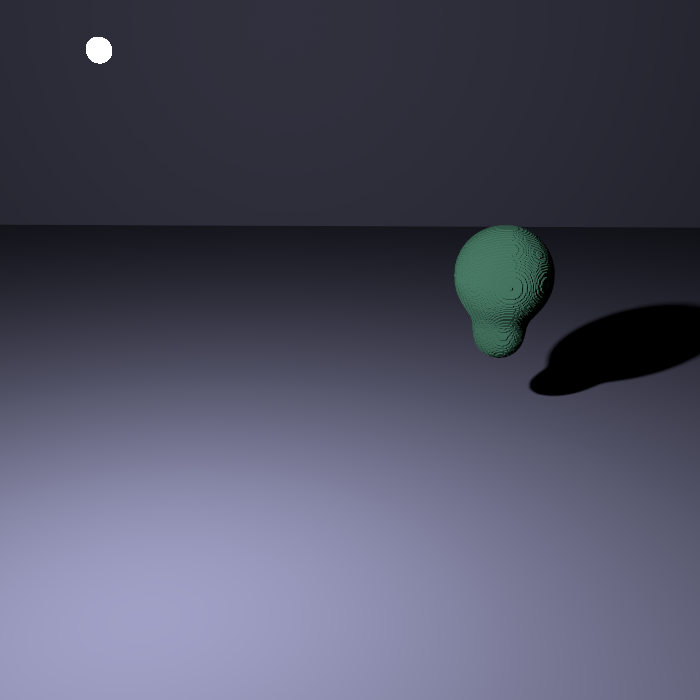
\includegraphics[width=1.0\textwidth]{imgs/metaball-preview.png}
          \end{center}
        \end{column}
      \end{columns}
    \end{frame}

    \begin{frame}
      \frametitle{Metaballs}
      \begin{itemize}
        \item Definidas de forma geral no $\mathbb{R}^n$
        \item Aqui com $F:\mathbb{R}^3 \to \mathbb{R}$
        \vspace{.5em}
        \begin{center}
          $F(x) = D(x) - T$
        \end{center}
        \begin{itemize}
          \item $D(x)$: soma das exponenciais
            \vspace{-1.0em}
            \begin{center}
              $$D(x) = \sum_{i = 1}^n Te^{\frac{B_i}{R_i^2}||x-P_i||^2-B_i} $$
            \end{center}
          \item $T$ - threshold
          \item $B_i$ - Blobbiness
          \item $R_i$ - Raio
        \end{itemize}
      \end{itemize}
    \end{frame}
      
    \begin{frame}
      \frametitle{Metaballs}
        \begin{center}
          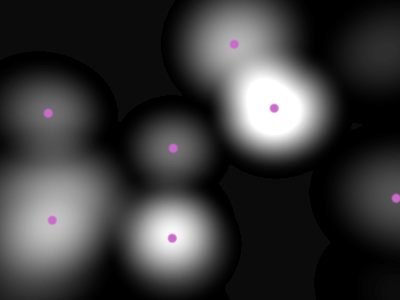
\includegraphics[width=.7\textwidth]{imgs/metaball-2d-1.png}
        \end{center}
    \end{frame}

    \begin{frame}
      \frametitle{Metaballs}
        \begin{center}
          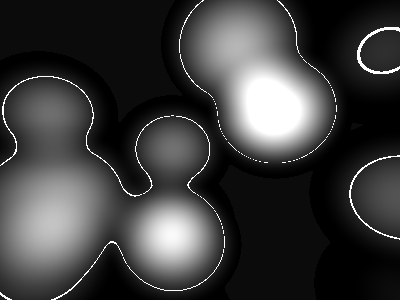
\includegraphics[width=.7\textwidth]{imgs/metaball-2d-2.png}
        \end{center}
    \end{frame}

    \begin{frame}
      \frametitle{Metaballs}
        \begin{center}
          
\includegraphics[width=.7\textwidth]{imgs/metaball-2d-3.png}
        \end{center}
    \end{frame}

    % Efeito dos parâmetros

  
        
  \section{Gerando uma mesh}
  
    \subsection{}
    
      \begin{frame}
        \frametitle{Resultado parcial}
        \begin{center}
          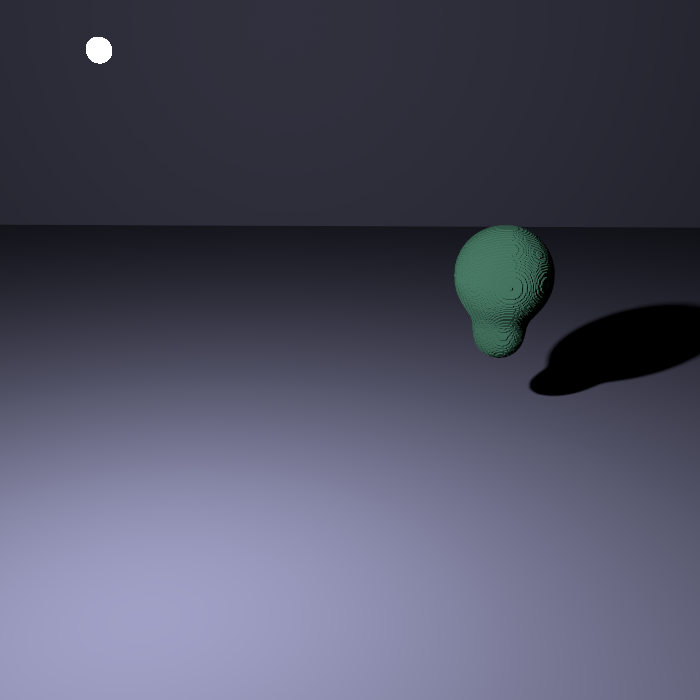
\includegraphics[width=.6\textwidth]{imgs/metaball-preview.png}
        \end{center}
      \end{frame}
  
\end{document}
